\section{CUDA Implementation}

\begin{frame}{GPU implementation - Introduction}
    \only<1>{
        \centering
        \Huge We've seen haswell .. \\
        \Huge \textbf{now back to the future !}
    }

    \only<2>{
        % Let's pretend we're in 2020
        % NVIDIA just released the A100, fastest GPU in the world
        \centering
        \textbf{The year is 2020 and NVIDIA just released their lastest GPU: The A100.}
        \begin{columns}

            \begin{column}{0.5\textwidth}
                \begin{figure}
                    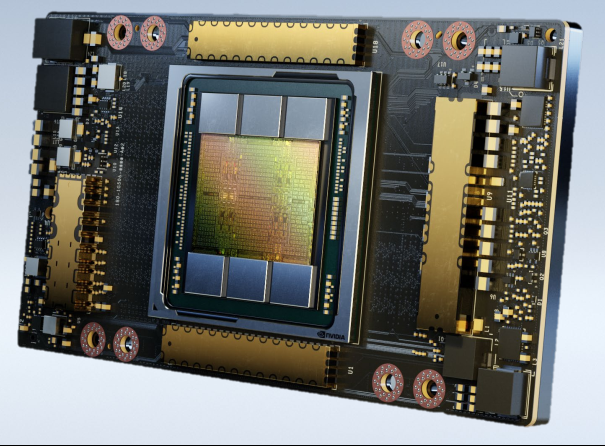
\includegraphics[width=.8\textwidth]{assets/A100_SXM4.png}
                    \captionof{figure}{NVIDIA A100 GPU}
                \end{figure}
            \end{column}

            \begin{column}{0.5\textwidth}
                \begin{figure}
                    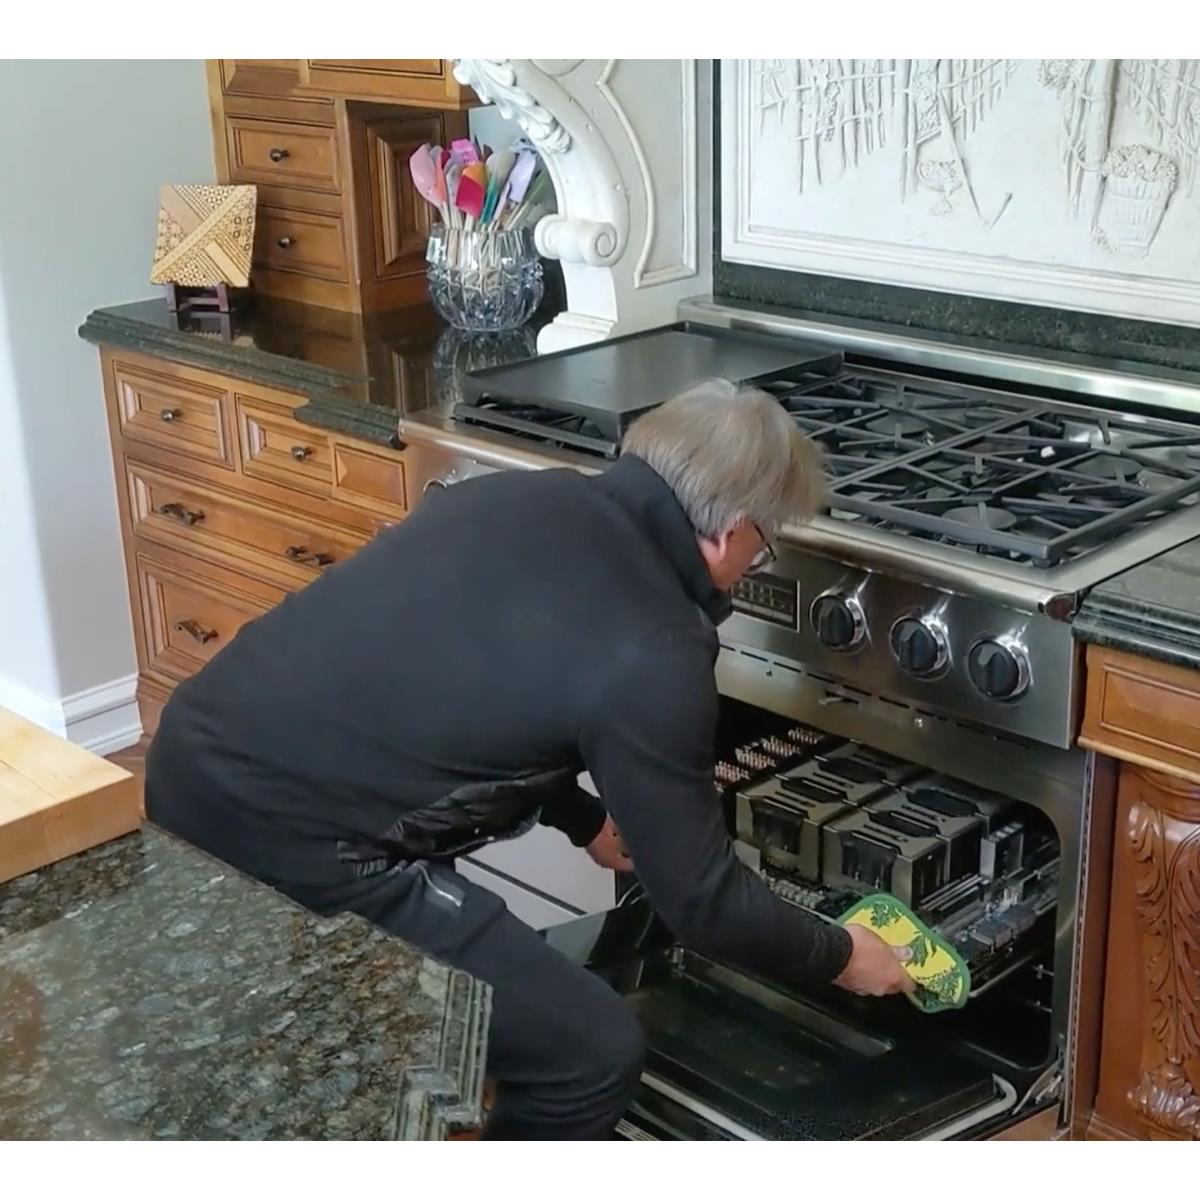
\includegraphics[width=.8\textwidth]{assets/jensen_oven.png}
                    \captionof{figure}{Jensen Huang cooking up a good card}
                \end{figure}
            \end{column}
        \end{columns}
    }

    % \only<3>{
    %     \begin{figure}
    %         \centering
    %         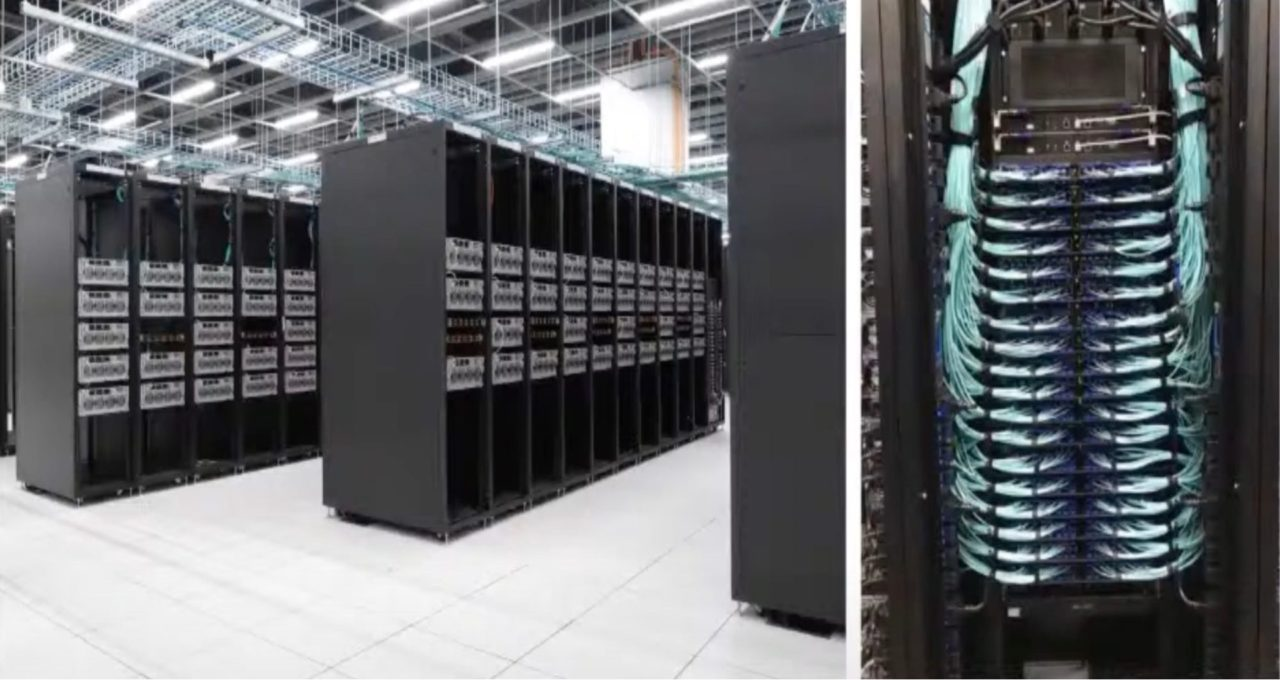
\includegraphics[width=\textwidth]{assets/A100_cluster.jpg}
    %         \captionof{figure}{NVIDIA A100 cluster (Tesla's)}
    %     \end{figure}
    % }
\end{frame}

\begin{frame}[t]{GPU implementation - Introduction}
    \textbf{What are we working with ?}

    \only<1>{
    \begin{itemize}
        \item \textbf{Tensor cores:} First GPU with FP64 GEMM hardware acceleration
        \item \textbf{Asynchronous copies:} Allows explicit pipelining
        \item \textbf{More power!} 108 SMs and 1.5TB/s of bandwidth, 19.5 TFlops in FP64!
        \item \textbf{NVLink 3.0:} Very fast D2D transfers !
    \end{itemize}
    }

    \only<2>{
    \begin{itemize}
        \item \textbf{Tensor cores:} First GPU with FP64 GEMM hardware acceleration
        \item \textbf{Asynchronous copies:} Allows explicit pipelining
        \item \textbf{More power!} 108 SMs and 1.5TB/s of bandwidth, \textbf{19.5 TFlops} in FP64!
        \item \sout{\textbf{NVLink 3.0:} Very fast D2D transfers !}
    \end{itemize}

    \textbf{Lots of useful features for us !}
    }
\end{frame}

% \begin{frame}{Targeting High-Performance DGEMM}
%     \begin{itemize}
%         \item \textbf{The Goal:} implement a high-performance Double Precision GEMM (DGEMM)
%         \item \textbf{Hardware Acceleration:} modern NVIDIA GPUs use \textbf{Tensor Cores} for peak performance
%         \item \textbf{The Catch:} FP64 Tensor Core acceleration is only on Data Center chips:
%         \begin{itemize}
%             \item \textbf{GA100} (A100), \textbf{GH100} (H100), \textbf{GB100} (Blackwell)
%         \end{itemize}
%     \end{itemize}
% \end{frame}
%
% \begin{frame}{Why Hardware Acceleration is Essential}
%     \begin{columns}
%         \begin{column}{0.5\textwidth}
%             \begin{itemize}
%                 \item \textbf{Standard FP64:} 9.7 TFLOPS
%                 \item \textbf{Tensor Core FP64:} 19.5 TFLOPS
%                 \item \textbf{The Gap:} $2\times$ performance increase just by using the right hardware instructions
%                 \item Without Tensor Cores, memory bandwidth dominates and optimization headroom is minimal
%             \end{itemize}
%         \end{column}
%         \begin{column}{0.5\textwidth}
%             \begin{center}
%                 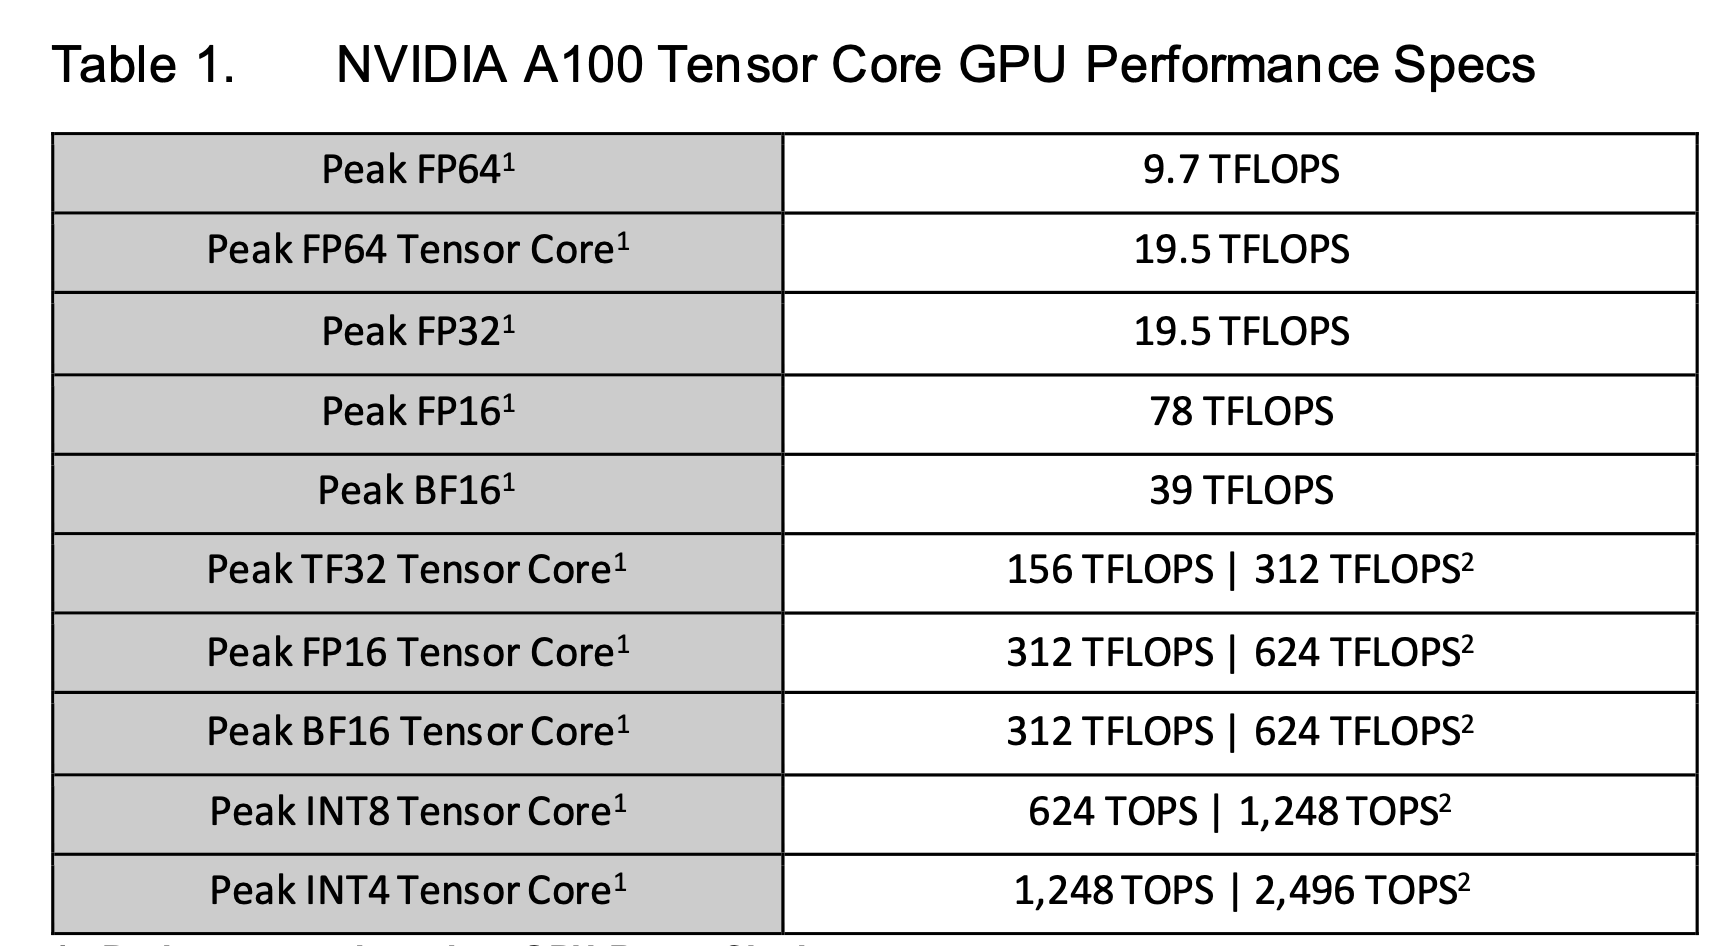
\includegraphics[width=\textwidth]{assets/a100_specs.png}
%                 \captionof{figure}{NVIDIA A100 Performance Specifications}
%             \end{center}
%         \end{column}
%     \end{columns}
% \end{frame}

\begin{frame}{Hardware Acceleration: Tensor Cores}

    \begin{columns}
        \begin{column}{0.6\textwidth}
            \textbf{But what is a tensor core ?}
            \begin{itemize}
                \item small hardware unit which performs fixed size GEMMs
                \item \textbf{Operation:} $D = A \times B + C$
                \item 4 tensor cores per SM (not as many as threads)
            \end{itemize}
        \end{column}
        \begin{column}{0.4\textwidth}
            \begin{center}
                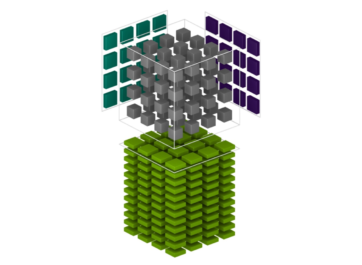
\includegraphics[width=.9\textwidth]{assets/tensor_core_illustration.png}
                \captionof{figure}{NVIDIA's illustration of a tensor core}
            \end{center}
        \end{column}
    \end{columns}
\end{frame}

\begin{frame}{Abstractions with NVIDIA CuTe}
    \begin{itemize}
        \item \textbf{The Problem:} Manual indexing is error-prone (even more with TCs)
        \item \textbf{The Solution:} \textbf{CuTe} (part of CUTLASS 3.0+)
        \item \textbf{Three main helpers:}
        \begin{itemize}
            \item \textbf{Layouts:} Mapping \textbf{logical coords} $\rightarrow$ \textbf{offset}
            \item \textbf{Tensors:} Composition of a Layout with some data (i.e: a pointer)
            \item \textbf{Tiled Operations:} Abstractions for tiling \textbf{Copies} and \textbf{MMAs}
        \end{itemize}
        \item \textbf{Benefit:} Allows us to focus on the algorithmic tiling strategy rather than pointer arithmetic
    \end{itemize}
\end{frame}

\begin{frame}{First Step: The "Naive" Baseline}
    \begin{columns}
        \begin{column}{0.5\textwidth}
            \begin{itemize}
                \item \textbf{Goal:} write a minimal GEMM kernel using FP64 TCs
                \item \textbf{Target:} NVIDIA A100 (GA100)
                \item \textbf{Key Components:}
                \begin{itemize}
                    \item \textbf{ALU:} FP64 Tensor Cores
                    \item \textbf{Tile Size:} Matches the atom size ($8 \times 8 \times 4$)
                    \item \textbf{Data Movement:} Used \texttt{cp.async}
                \end{itemize}
            \end{itemize}
        \end{column}
        \begin{column}{0.5\textwidth}
            \begin{center}
                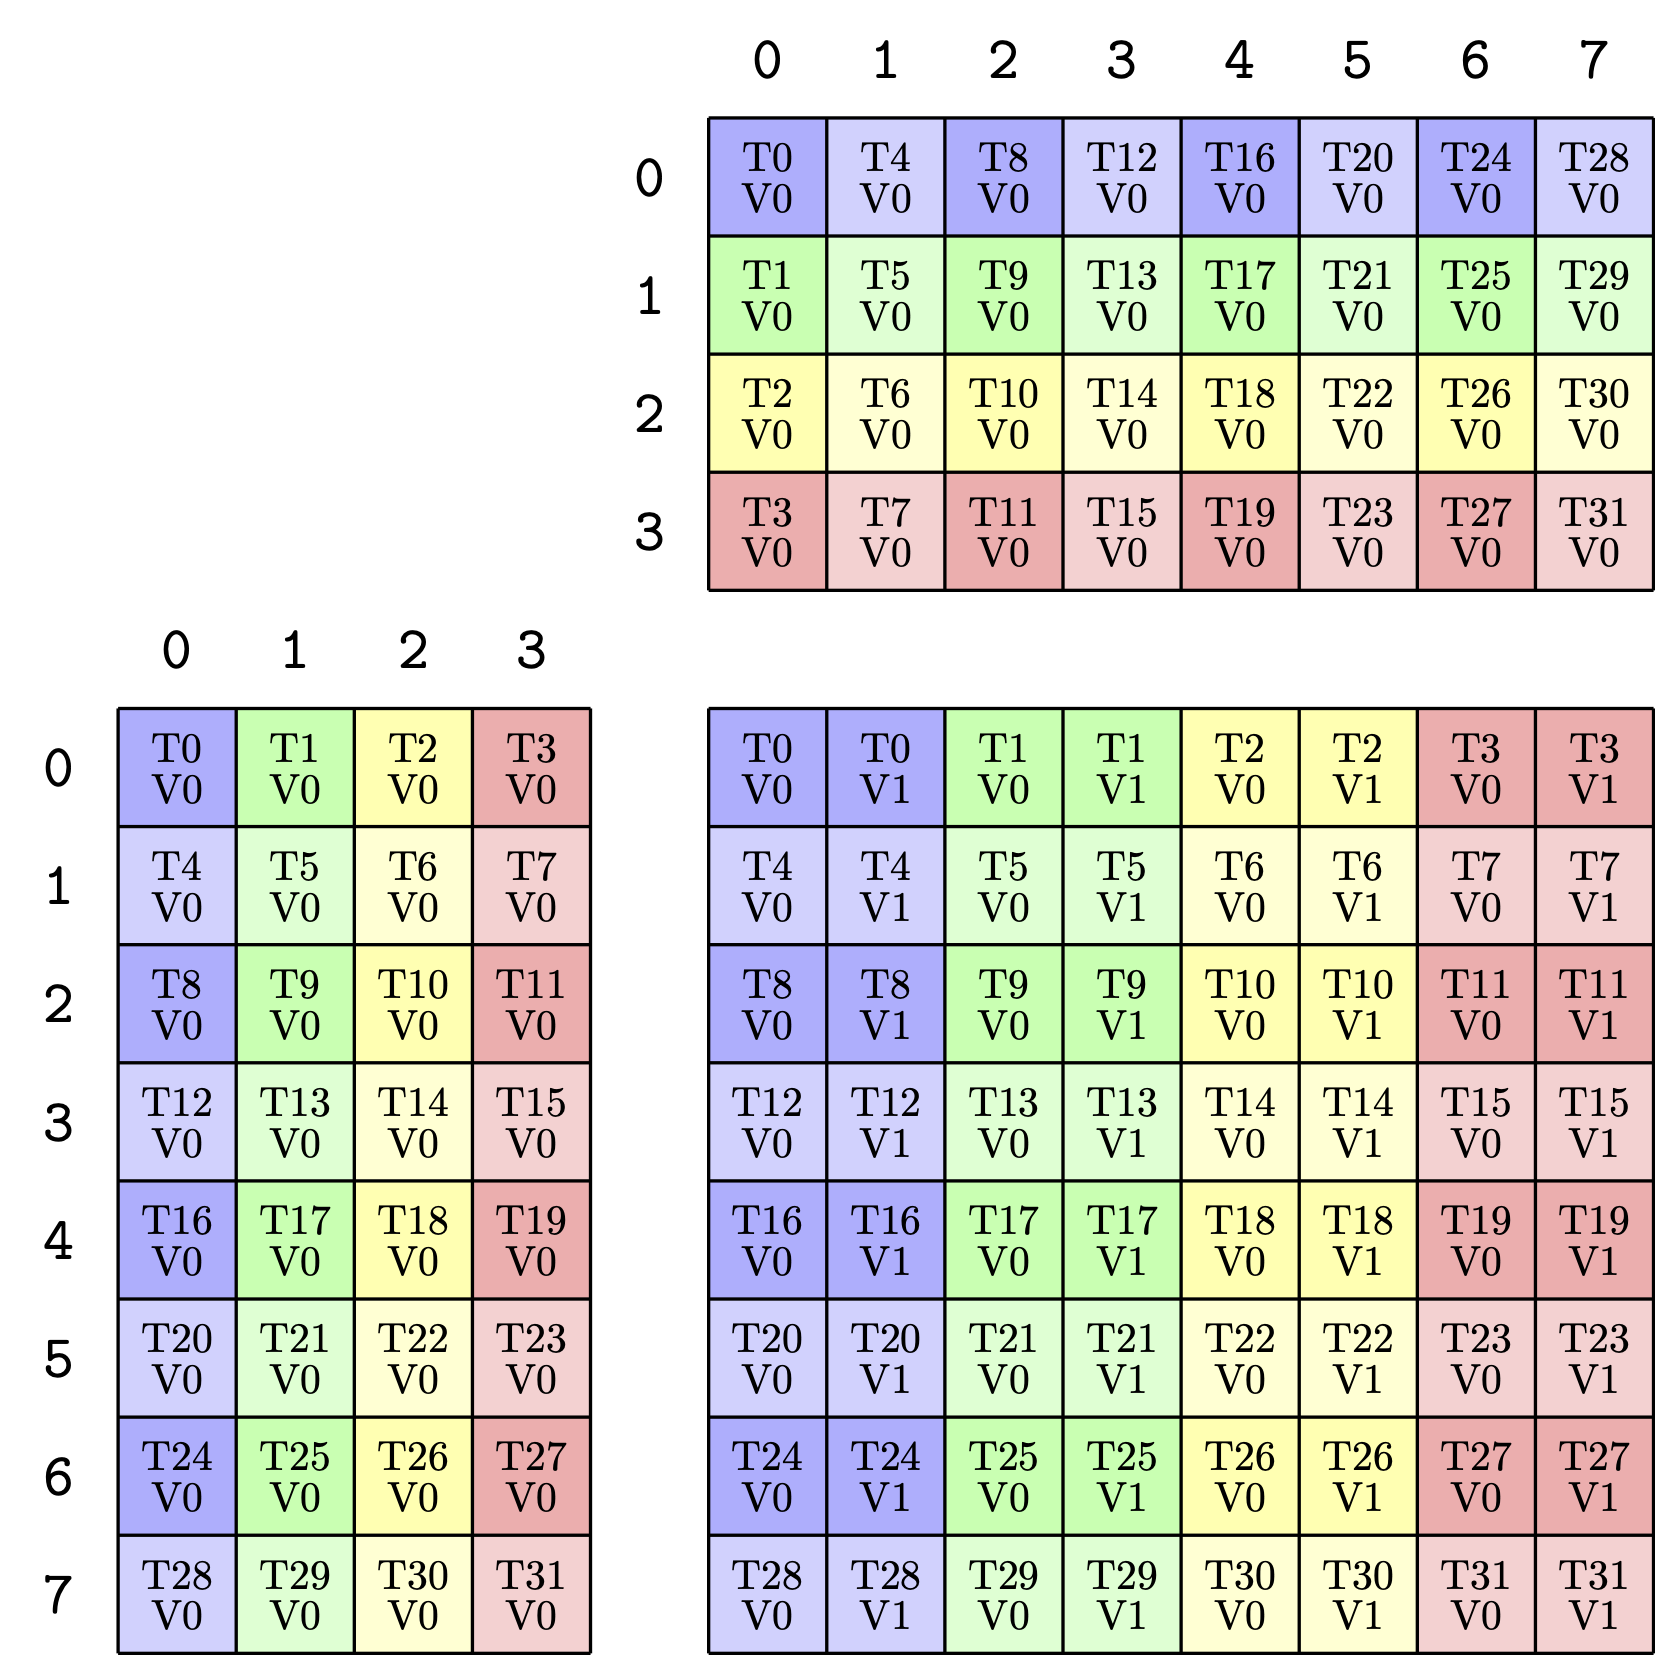
\includegraphics[width=.9\textwidth]{assets/m8n8k4.png}
                \captionof{figure}{\texttt{SM80\_8x8x4\_F64F64F64F64\_TN} MMA Atom}
            \end{center}
        \end{column}
    \end{columns}
\end{frame}

\begin{frame}[t]{Baseline: Results}
    \begin{center}
        \includegraphics[height=.80\textheight]{res/cuda_baseline_16:9.png}
        %\captionof{figure}{Baseline benchmark}
    \end{center}
\end{frame}

\begin{frame}{Optimization: Larger TiledMMA}
    \begin{columns}
        \begin{column}{0.5\textwidth}
            \begin{itemize}
                \item \textbf{Goal:} Increate arithmetic intensity
                \item \textbf{Solution:} Use a larger tensor core atom. We can duplicate the current atom accross K dimension
            \end{itemize}
        \end{column}
        \begin{column}{0.5\textwidth}
            \begin{center}
                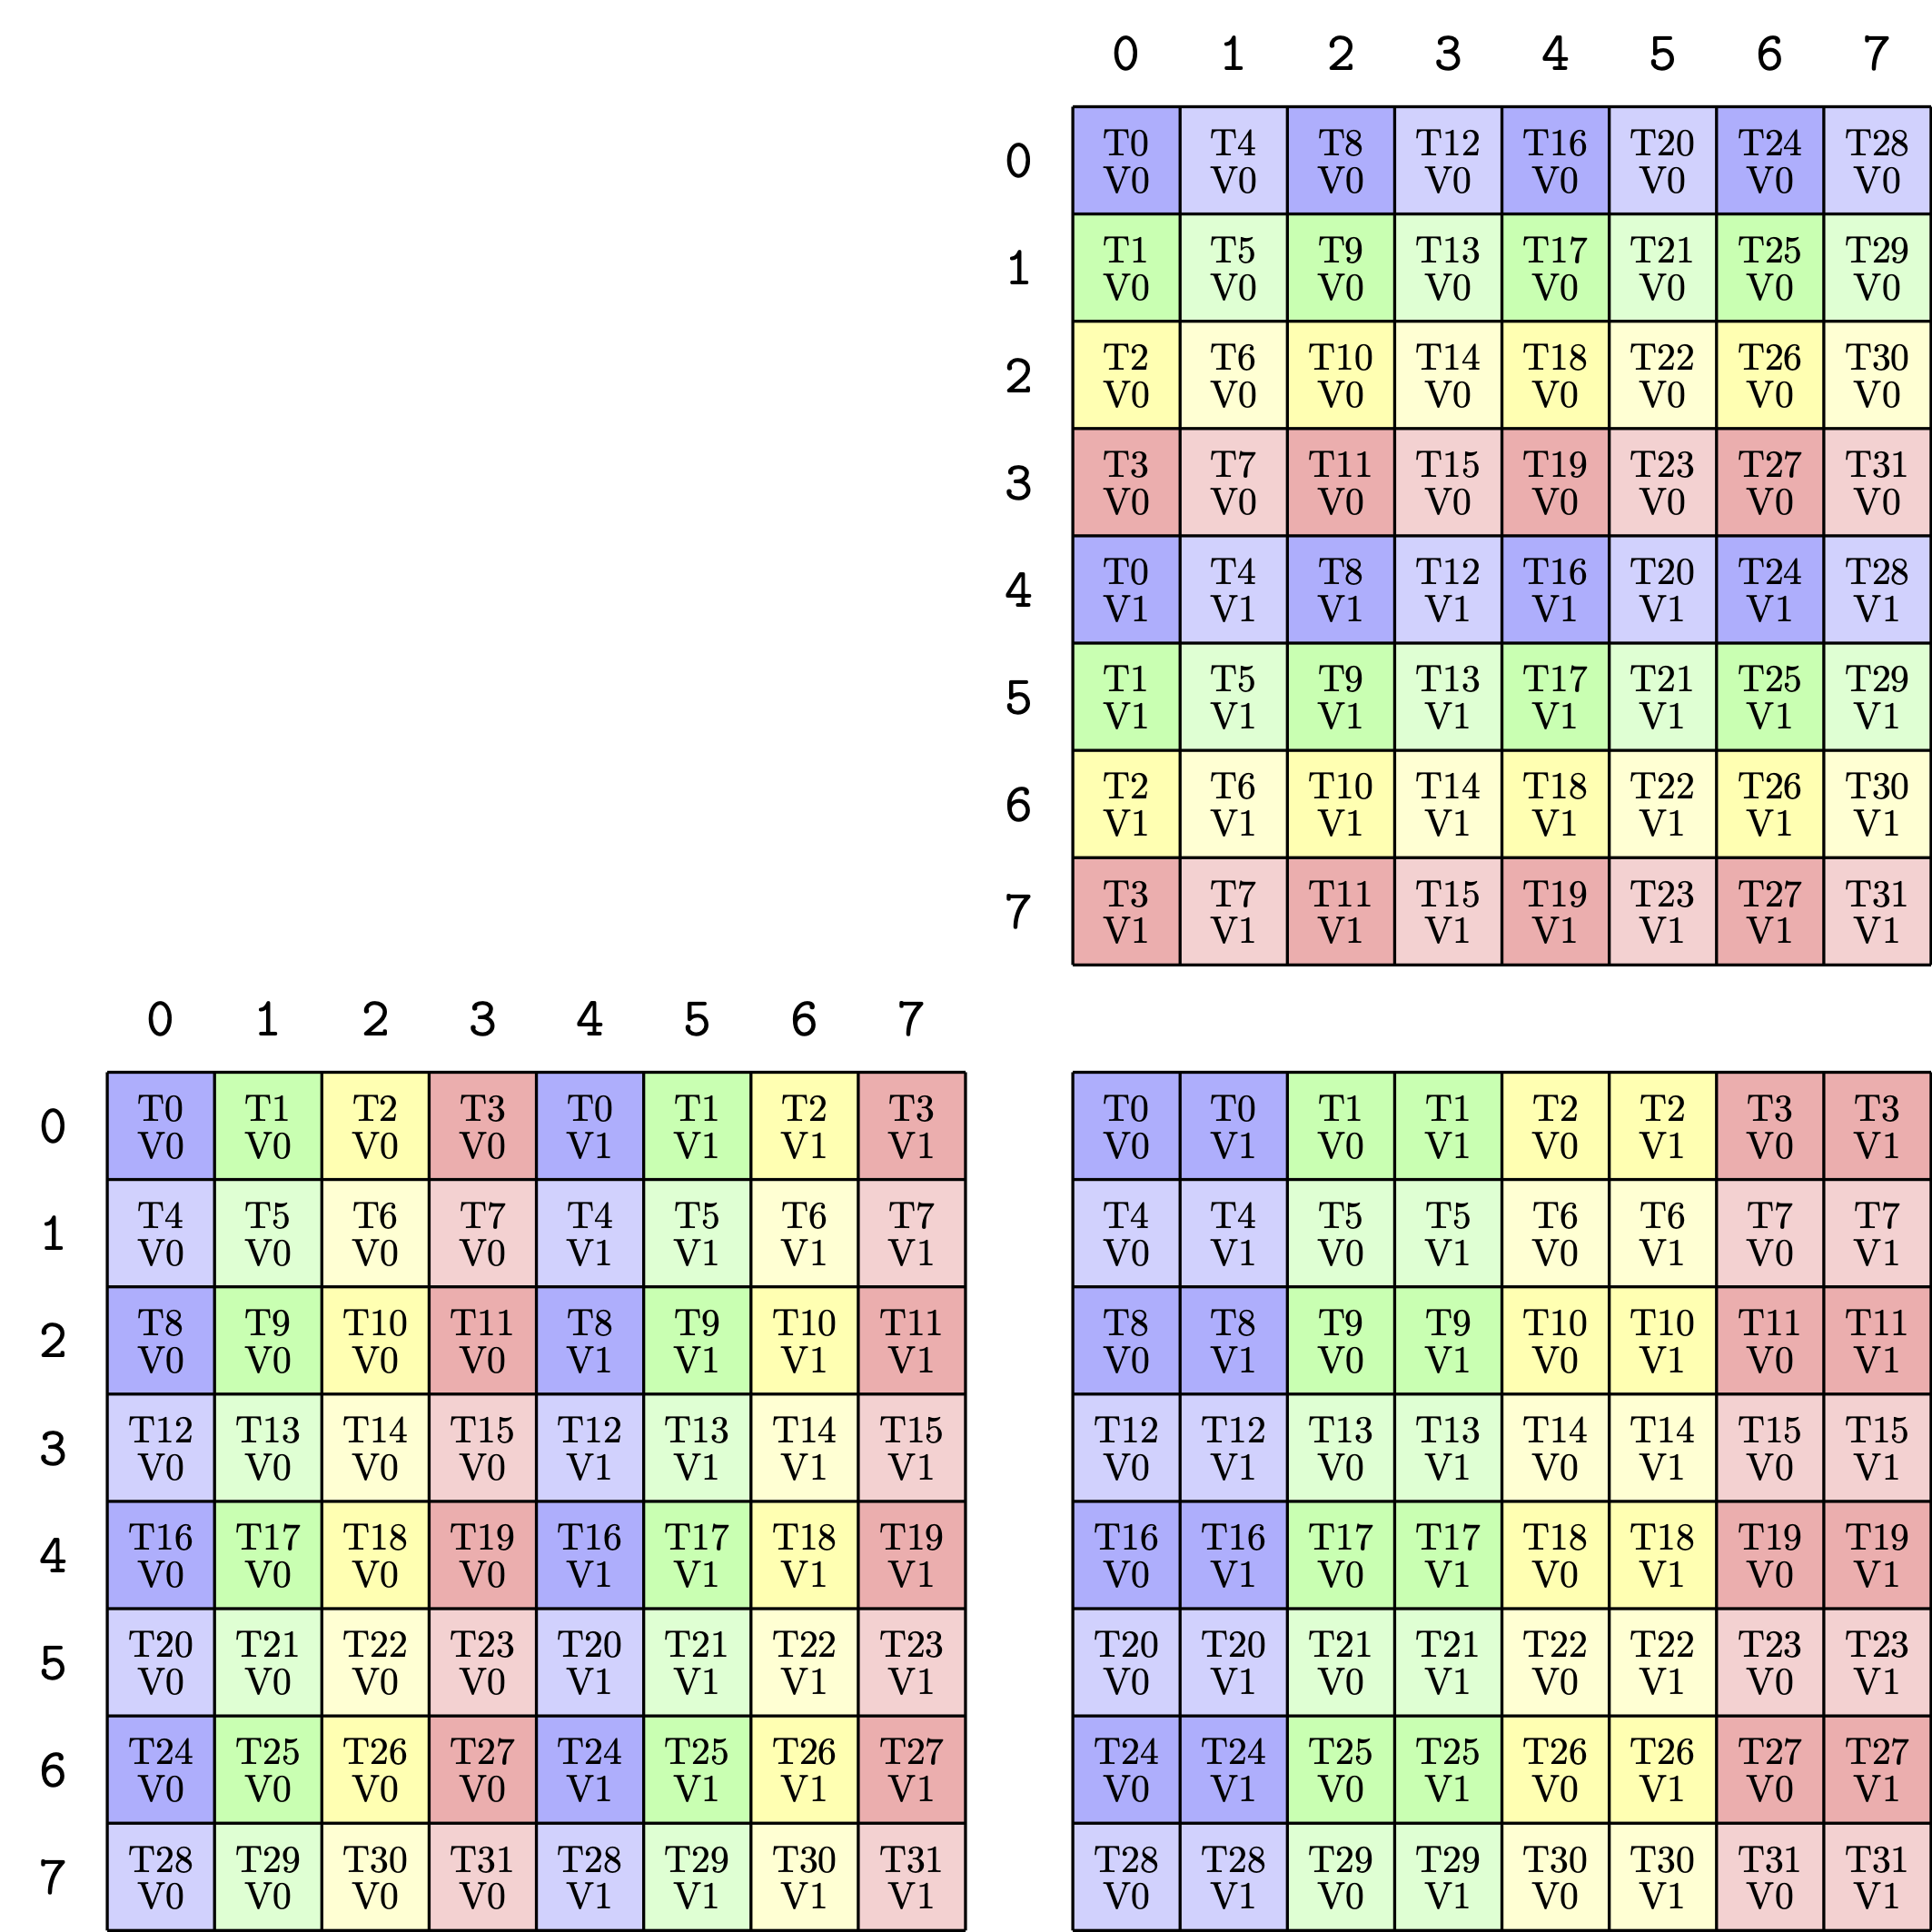
\includegraphics[width=\textwidth]{assets/m8n8k8.png}
                \captionof{figure}{m8n8k8 tiled MMA atom}
            \end{center}
        \end{column}
    \end{columns}
\end{frame}

\begin{frame}[t]{Larger TiledMMA optimization: Results}
    \begin{center}
        \includegraphics[height=.80\textheight]{res/cuda_baseline_m8n8k8_16:9.png}
        %\captionof{figure}{cuda\_baseline\_m8n8k8 benchmark}
    \end{center}
\end{frame}

\begin{frame}{Optimization: Vectorized copies}
    \begin{itemize}
        \item \textbf{Problem:} We are still memory bound
        \item \textbf{Solution:} Copy larger blocks of data with a single copy instruction
    \end{itemize}

    \begin{center}
        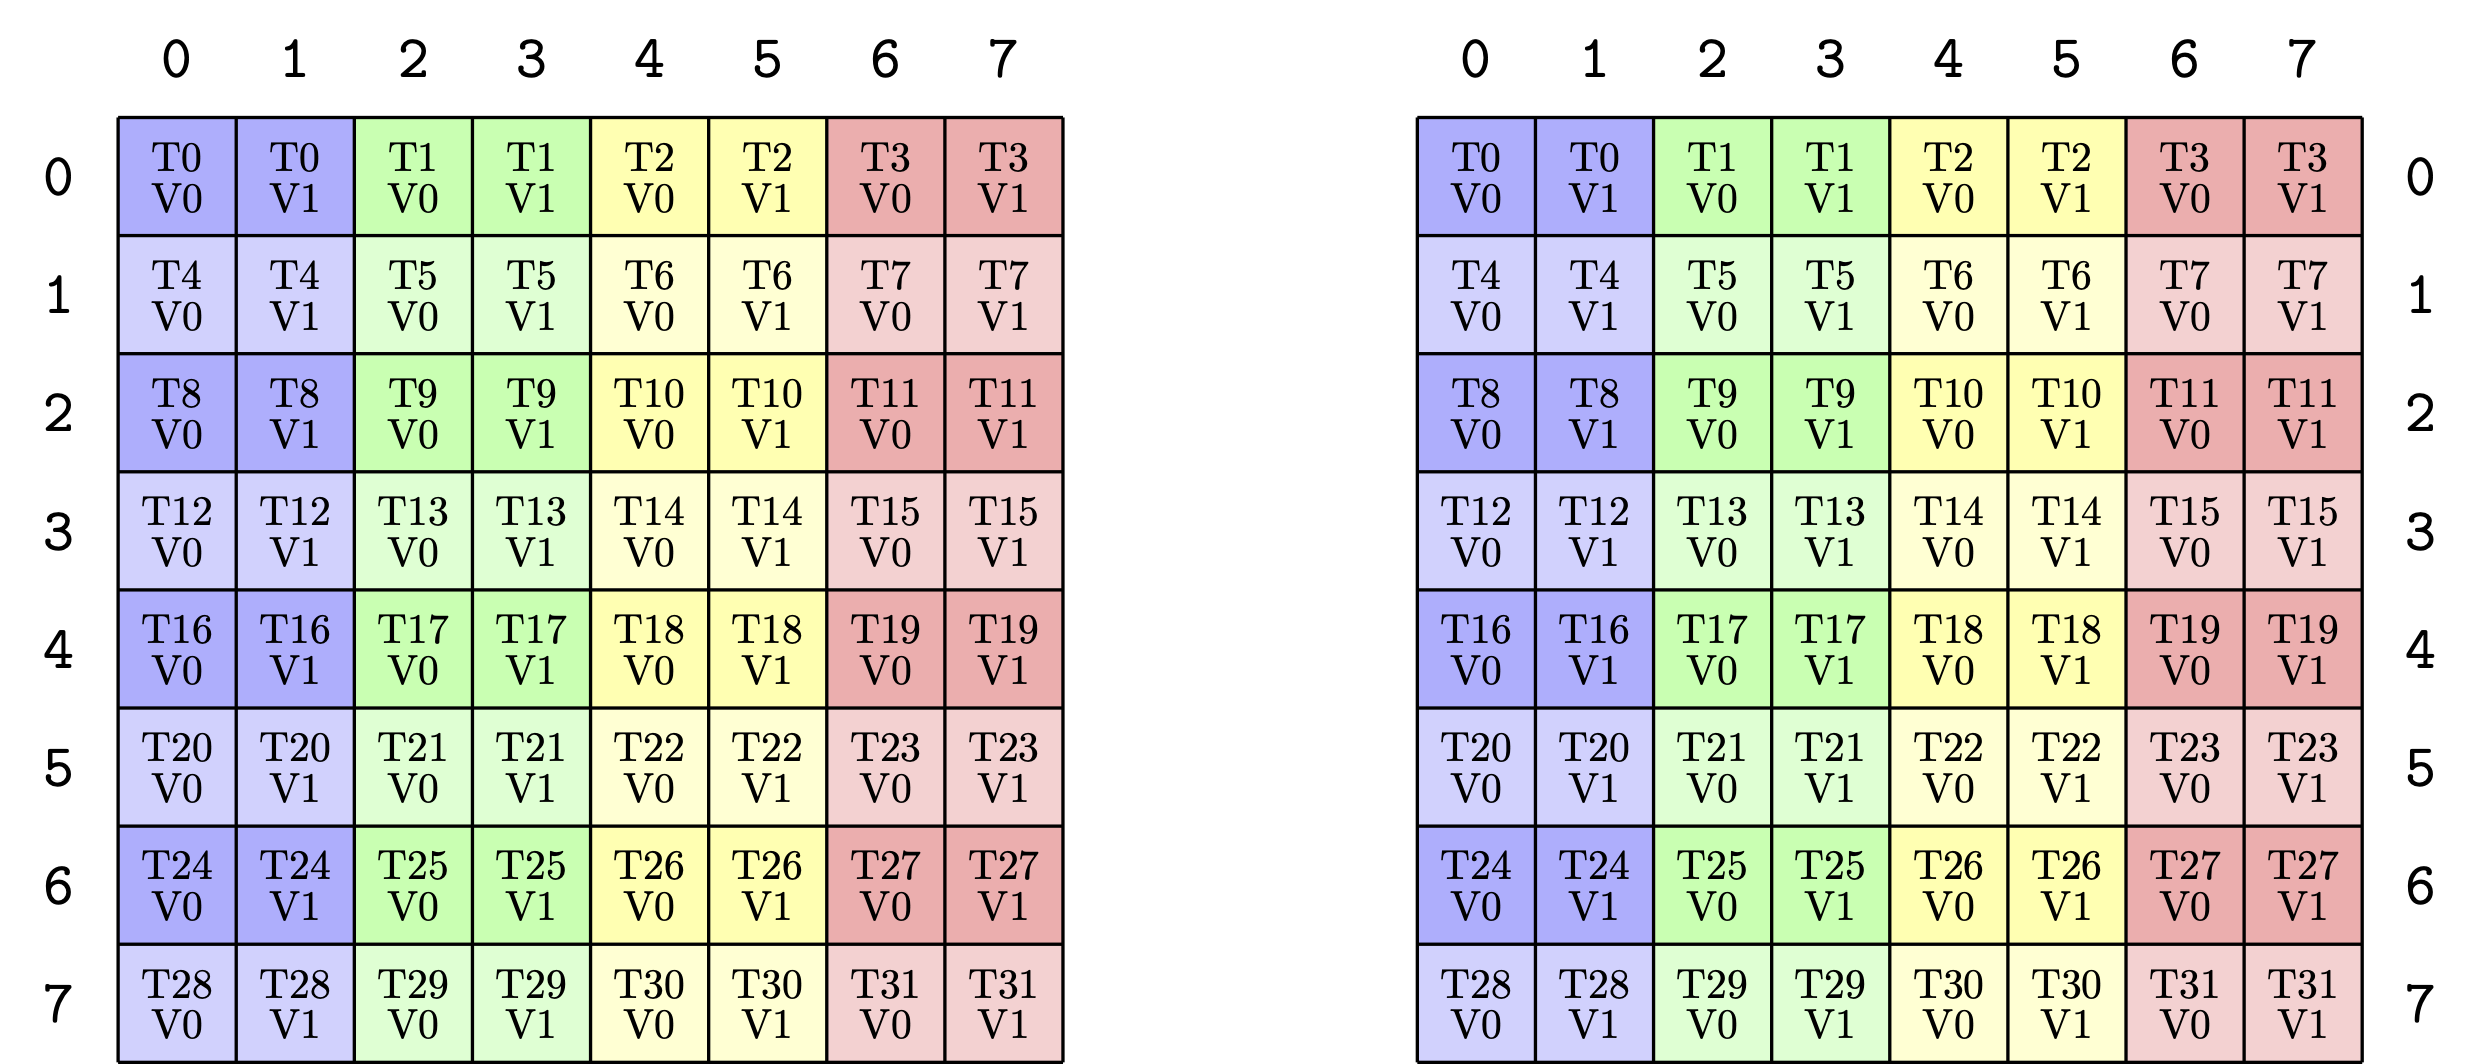
\includegraphics[width=0.7\textwidth]{assets/128b_cpy.png}
        \captionof{figure}{vectorized 128bit copy TiledCopy}
    \end{center}
\end{frame}
\begin{frame}[t]{Vectorized copies optimization: Results}
    \begin{center}
        \includegraphics[height=.80\textheight]{res/cuda_baseline_m8n8k8_128b_16:9.png}
        %\captionof{figure}{cuda\_baseline\_m8n8k8\_128b benchmark}
    \end{center}
\end{frame}

\begin{frame}{Optimization: Larger tiled MMA again}
    \begin{columns}
        \begin{column}{0.5\textwidth}
            \begin{itemize}
                \item \textbf{Problem:} We are using our memory subsystem as much as we can, we need to increase the arithmetic intensity for more flops
                \item \textbf{Solution:} Use a larger tiled MMA again
            \end{itemize}
        \end{column}
        \begin{column}{0.5\textwidth}
            \begin{center}
                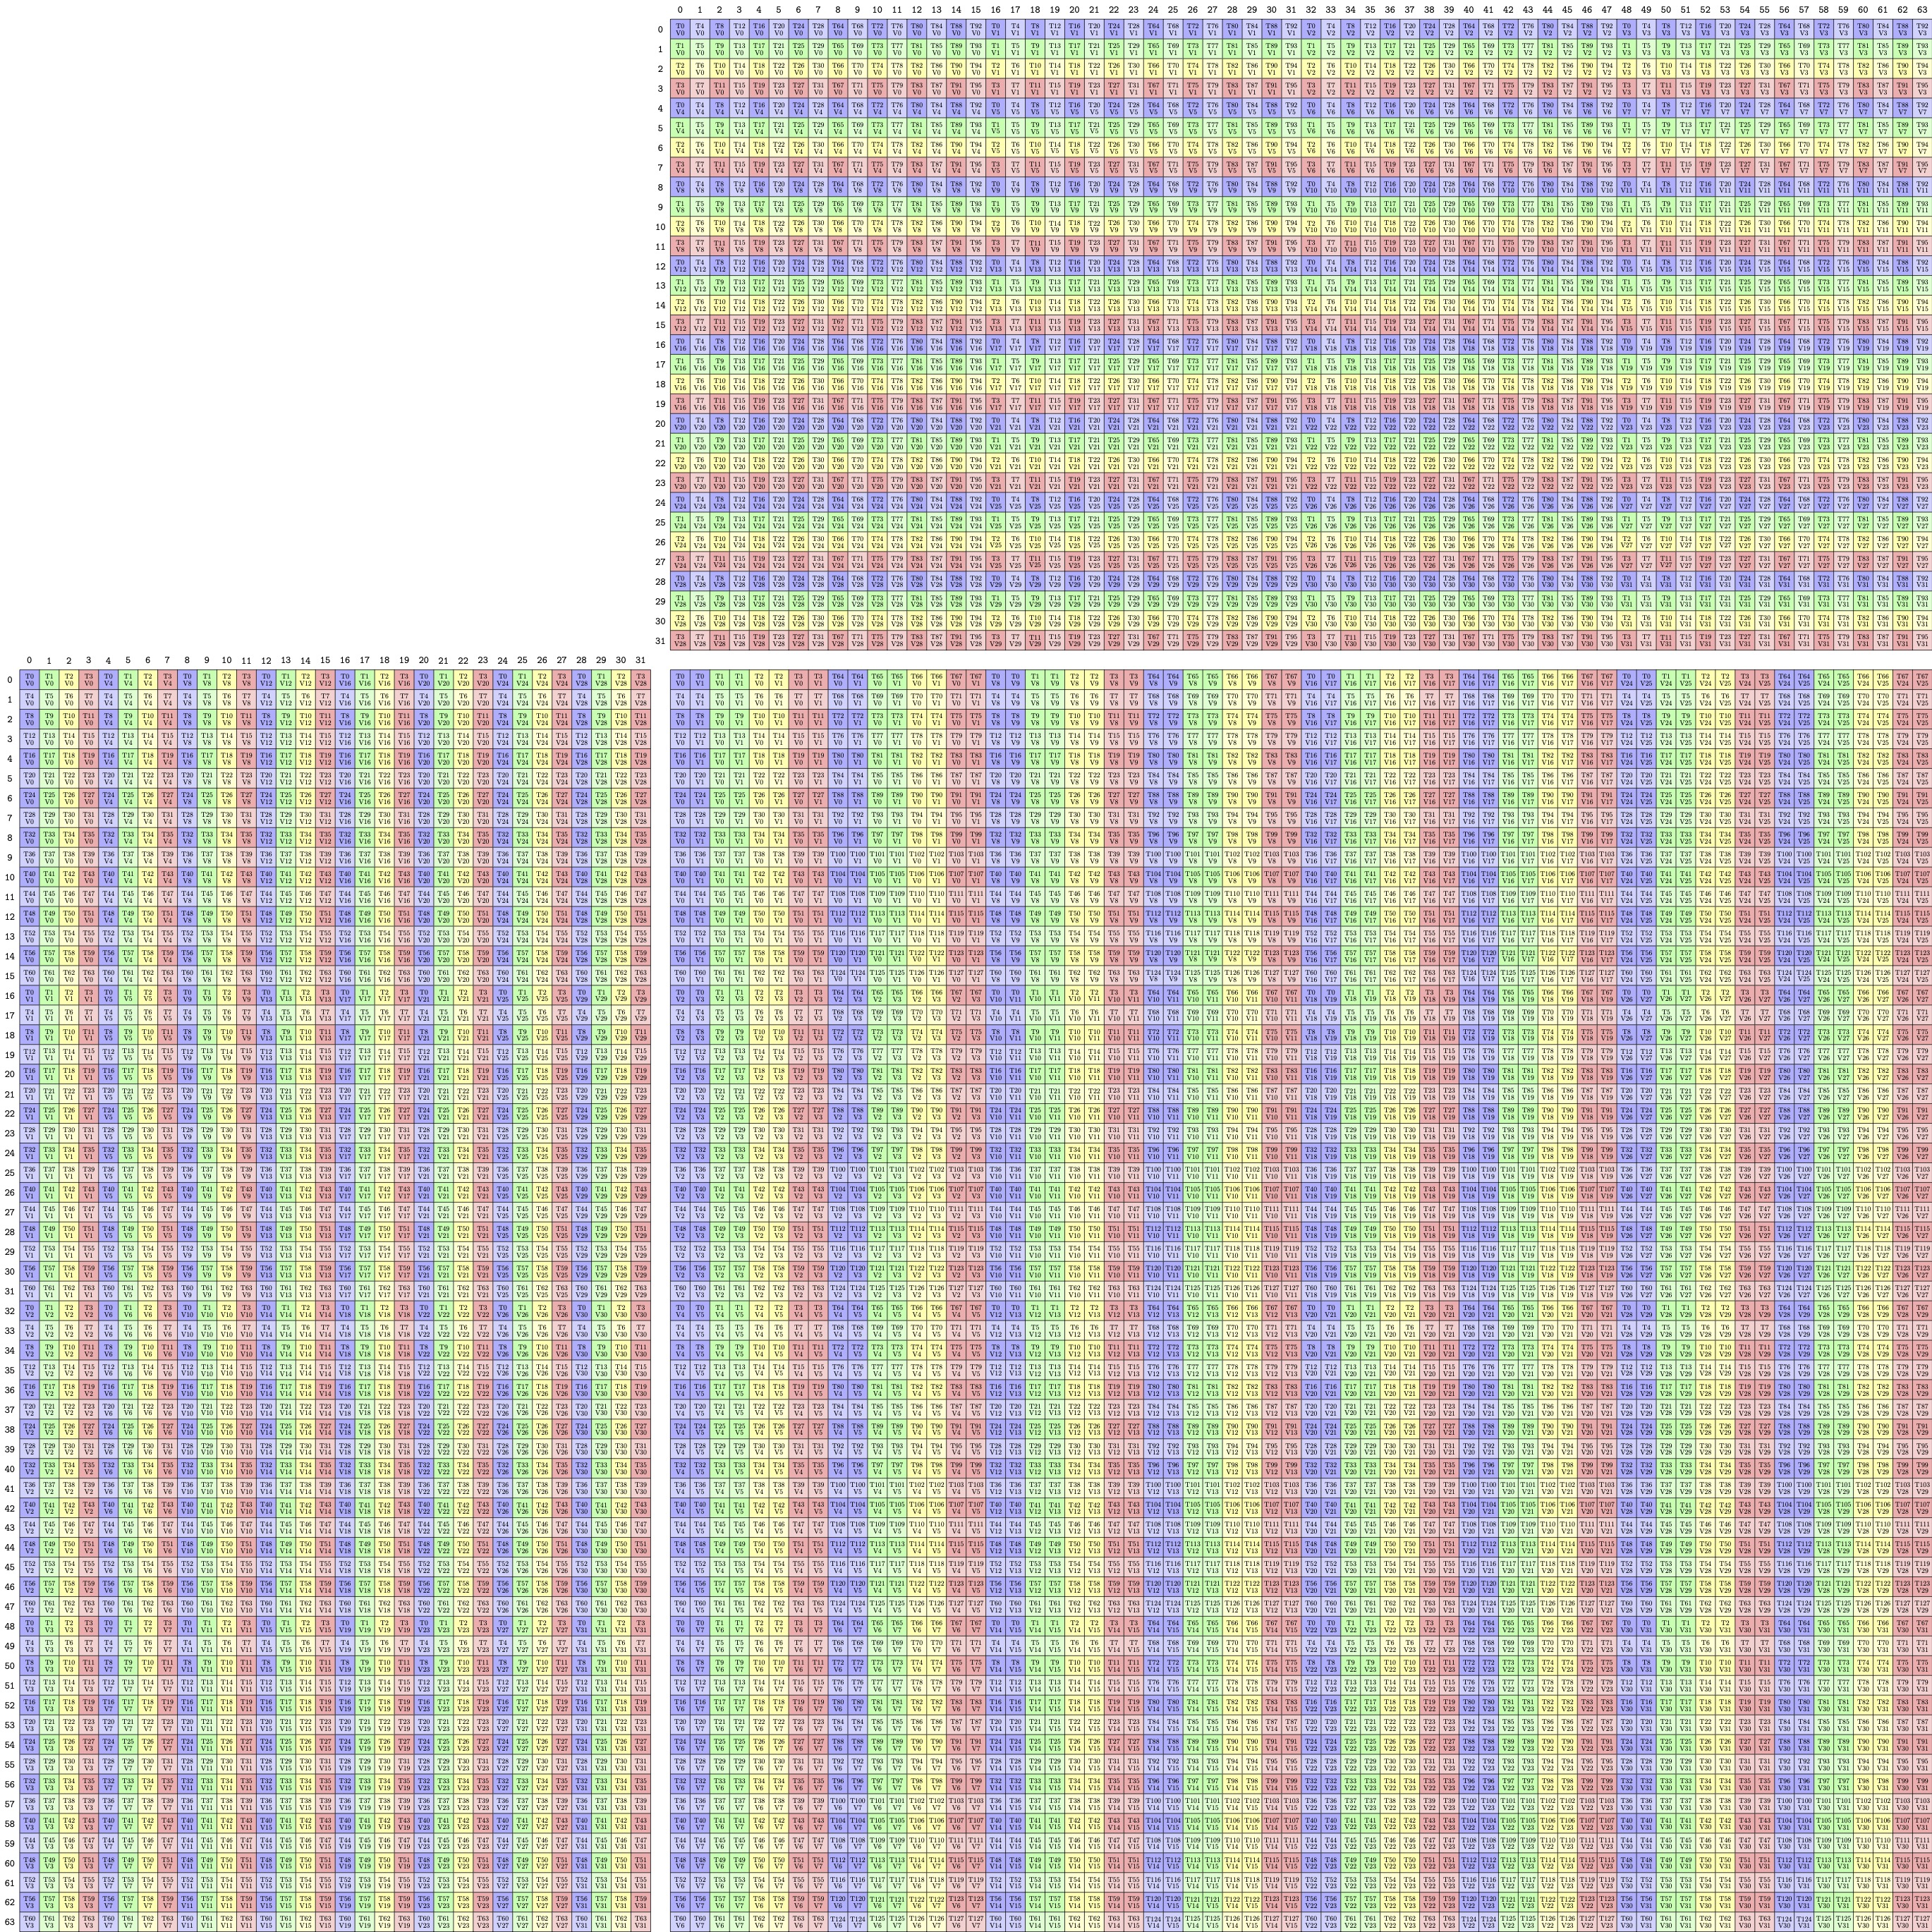
\includegraphics[width=\textwidth]{assets/m64n64k32.jpg}
                \captionof{figure}{m64n64k32 tiled MMA atom}
            \end{center}
        \end{column}
    \end{columns}
\end{frame}
\begin{frame}[t]{Larger tiled MMA optimization: Results}
    \begin{center}
        \includegraphics[height=.80\textheight]{res/cuda_baseline_m64n64k32_128b_16:9.png}
        %\captionof{figure}{cuda\_baseline\_m64n64k32\_128b benchmark}
    \end{center}
\end{frame}

\begin{frame}{Optimization: Use the whole physical GPU core}
    \begin{columns}
        \begin{column}{0.6\textwidth}
            \begin{itemize}
                \item \textbf{Problem:} We are only using 1/4th of the physical GPU core (SM)
                \item \textbf{Solution:} Run the TiledMMA on each quadrant of the core. (block tiling)
            \end{itemize}
        \end{column}
        \begin{column}{0.4\textwidth}
            \begin{center}
                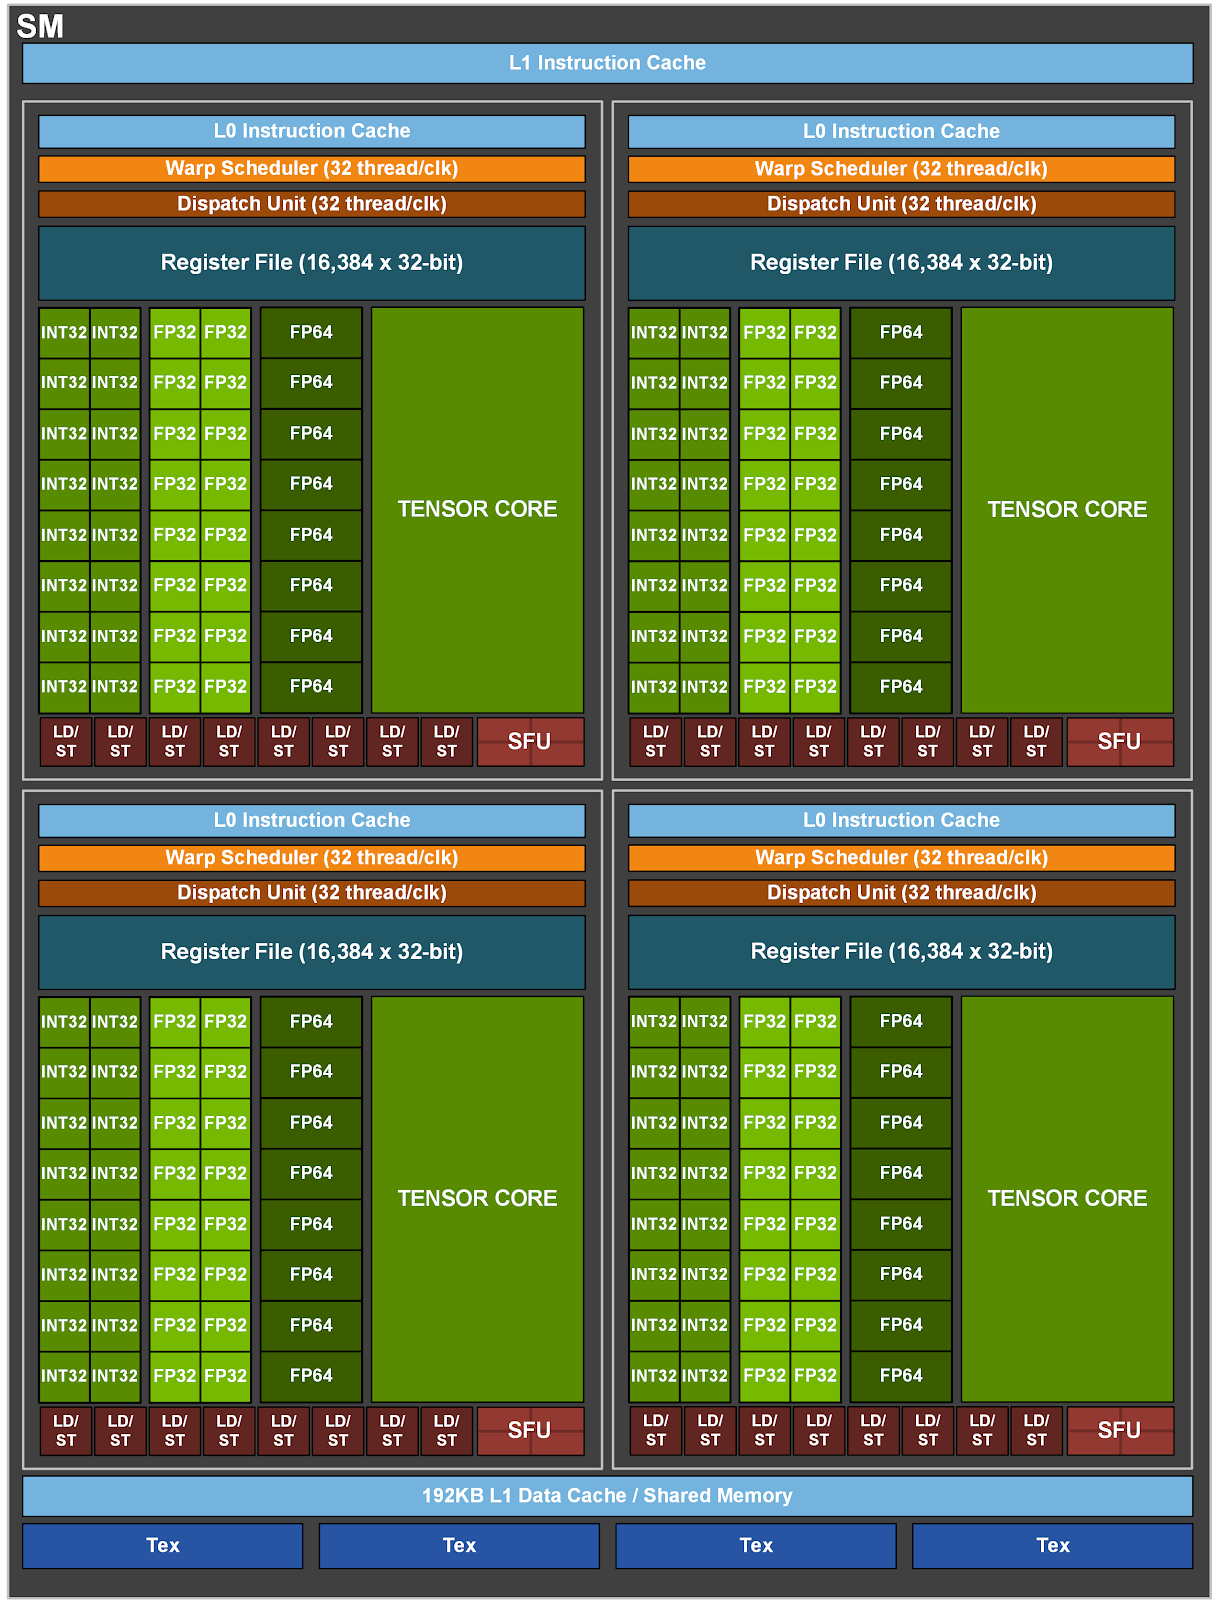
\includegraphics[width=.8\textwidth]{assets/A100_SM.png}
                \captionof{figure}{NVIDIA A100 core diagram (SM)}
            \end{center}
        \end{column}
    \end{columns}
\end{frame}
\begin{frame}[t]{Block tiling optimization: Results}
    \begin{center}
        \includegraphics[height=.80\textheight]{res/cuda_baseline_m64n64k32_128b_4W_16:9.png}
        %\captionof{figure}{cuda\_baseline\_m64n64k32\_128b\_4W benchmark}
    \end{center}
\end{frame}

\begin{frame}{Optimization: Caching policy}
    \begin{itemize}
        \item \textbf{Problem:} When looking at the data loading scheme, we notice that each block is loaded from global memory once. We are misusing our L1 cache
        \item \textbf{Solution:} Instruct the hardware to skip L1 when loading data from global memory
    \end{itemize}
\end{frame}
\begin{frame}[t]{Caching policy optimization: Results}
    \begin{center}
        \includegraphics[height=.80\textheight]{res/cuda_baseline_m64n64k32_128b_4W_CG_16:9.png}
        %\captionof{figure}{cuda\_baseline\_m64n64k32\_128b\_4W\_CG benchmark}
    \end{center}
\end{frame}
